\chapter{Analisis}
\label{chap:analisis}

\section{Analisis Sistem Kini}
\label{sec:3:analisiskini} 

Seperti dibahas pada bab \ref{chap:intro}, SharIF Judge adalah sebuah \textit{online judge} dengan fungsi utama untuk mengevaluasi kode program yang dikumpulkan oleh pengguna secara otomatis. SharIF Judge digunakan pada beberapa mata kuliah pemrograman Teknik Informatika Unpar untuk mempermudah proses pengumpulan dan penilaian kode program. SharIF Judge dibangun menggunakan PHP dengan \textit{framework} CodeIgniter dan Bash. 

\subsection{Istilah-istilah Umum}
\label{subs:3:assignment}

Pada SharIF Judge, digunakan istilah-istilah berikut ini:

\begin{itemize}
    \item \textit{Assignment} \\ Merepresentasikan sebuah tugas yang diberikan. Pada sebuah \textit{assignment}, ditentukan waktu mulai, tenggat waktu, partisipan, dan soal-soal yang diberikan. Untuk setiap \textit{assignment}, dapat diunggah sebuah \textit{file} PDF yang berisi seluruh soal, serta tes kasus dan jawaban yang digunakan untuk menilai kode.
    \item \textit{Problem} \\ Merepresentasikan sebuah soal yang terdapat pada \textit{assignment}. Untuk setiap \textit{problem}, dapat ditentukan ekstensi \textit{file} yang diizinkan, serta batas waktu dan memori kode. Sebuah \textit{problem} dapat bersifat \textit{upload only}, yang berarti \textit{file} jawaban hanya diunggah, namun tidak dinilai dengan tes kasus.
    \item \textit{Submission} \\ Merepresentasikan sebuah jawaban dari seorang pengguna untuk sebuah \textit{problem}. Untuk setiap \textit{submission}, pengguna mengunggah sebuah \textit{file} yang kemudian akan dinilai.
    \item \textit{Final Submission} \\ Merepresentasikan sebuah jawaban akhir dari seorang pengguna. Seorang pengguna dapat mengunggah \textit{submission} berkali-kali untuk menguji dan memperbarui jawaban, namun harus memilih satu buah \textit{submission} sebagai jawaban final.
\end{itemize}

\begin{figure}[H]
	\centering  
	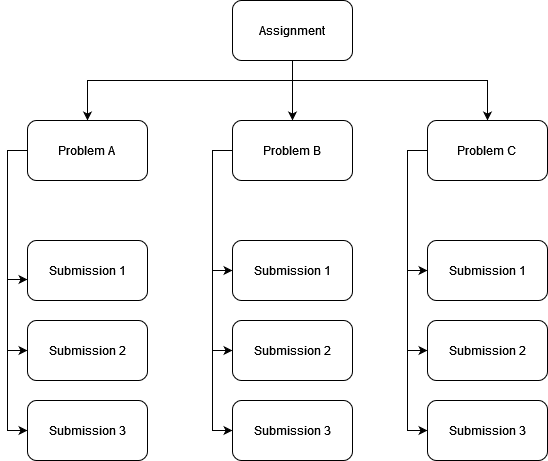
\includegraphics[scale=0.4]{Diagram/assignment.png}  
	\caption{Bagan hubungan \textit{assignment}, \textit{problem}, dan \textit{submission} pada SharIF Judge}
	\label{fig:3:assignment} 
\end{figure} 

Gambar \ref{fig:3:assignment} menunjukkan hubungan \textit{assignment}, \textit{problem}, dan \textit{submission} pada SharIF Judge. Sebuah \textit{assignment} dapat terdiri beberapa \textit{problem}. Untuk setiap \textit{problem}, pengguna dapat mengumpulkan \textit{submission} berkali-kali, lalu memilih salah satunya sebagai \textit{final submission}.

\subsection{Fitur-fitur SharIF Judge}
\label{subs:3:fitur}

    \begin{figure}[H]
    	\centering  
    	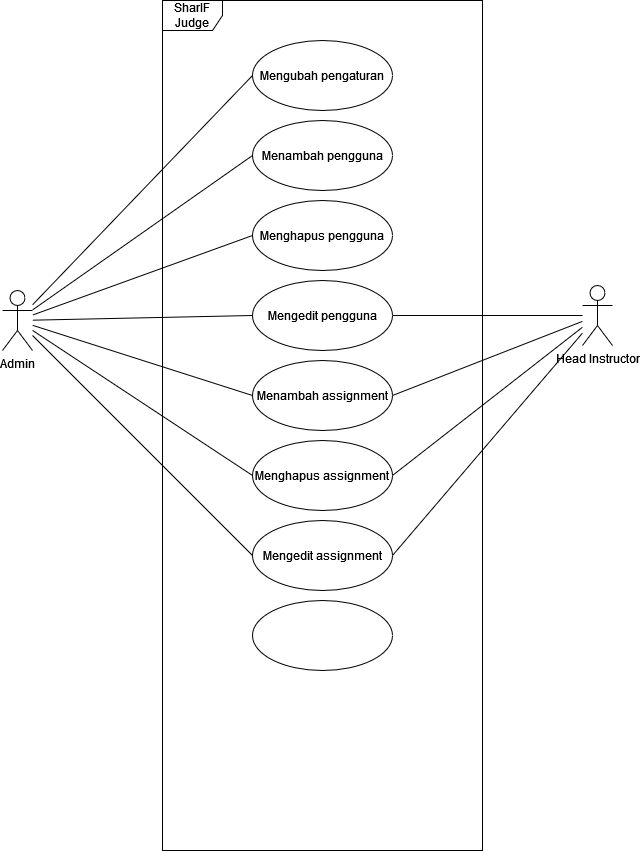
\includegraphics[scale=0.4]{Diagram/Use Case.png}  
    	\caption{Use Case Diagram SharIF Judge}
    	\label{fig:3:usecased} 
    \end{figure} 

Halaman dan tampilan yang tersedia pada pengguna SharIF Judge bergantung pada \textit{role} akun yang digunakan pengguna tersebut. Pada gambar \ref{fig:3:usecased}, terdapat Use Case Diagram untuk setiap \textit{role} yang tersedia. Berikut ini adalah setiap halaman dan fitur yang terdapat pada SharIF Judge untuk \textit{role} \textit{admin}:

\subsubsection{Dashboard}
    \begin{figure}[H]
    	\centering  
    	\includegraphics[scale=0.35]{Page/dashboard.PNG}  
    	\caption{Halaman Dashboard}
    	\label{fig:3:dashboard} 
    \end{figure} 
    
    Gambar \ref{fig:3:dashboard} menunjukkan halaman Dashboard. Pada halaman ini terdapat kalender yang menunjukkan durasi setiap \textit{assignment} dan daftar notifikasi.
    
\subsubsection{Settings}
    \begin{figure}[H]
    	\centering  
    	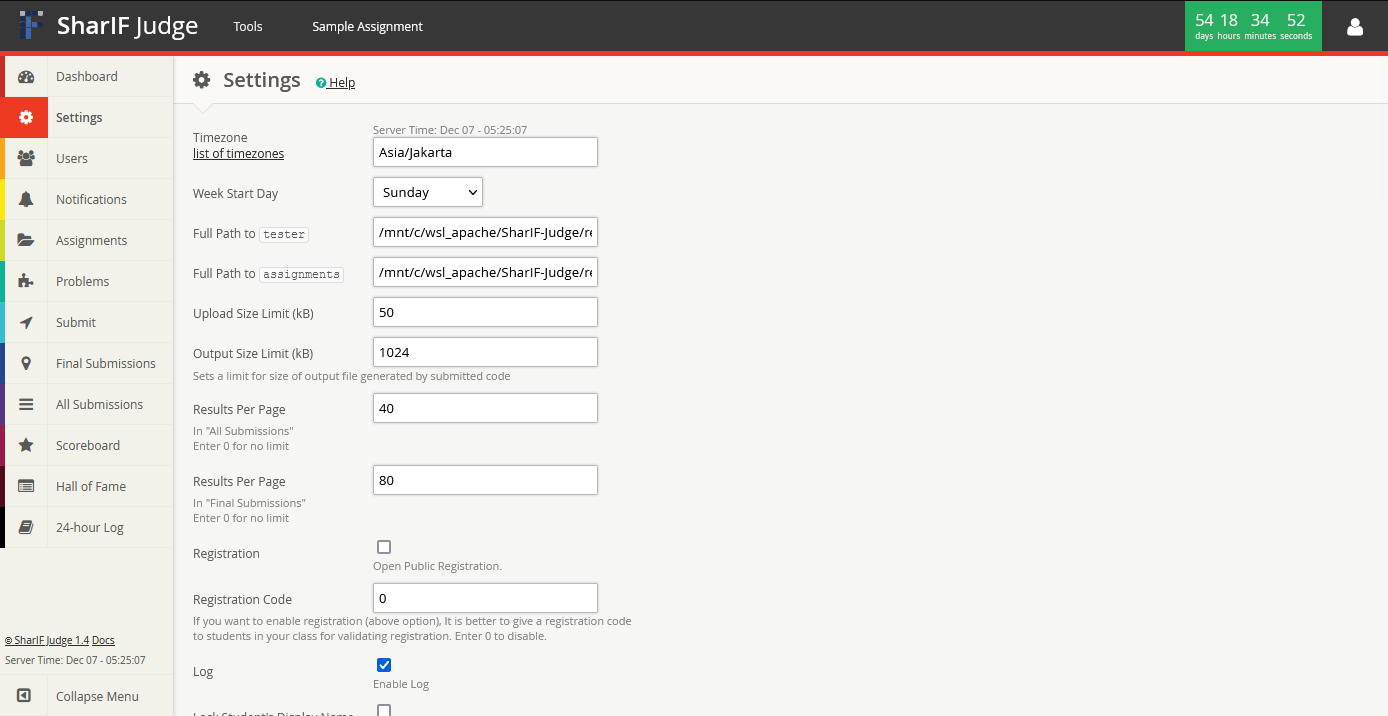
\includegraphics[scale=0.35]{Page/settings.PNG}  
    	\caption{Halaman Settings}
    	\label{fig:3:settings} 
    \end{figure} 
    
    Gambar \ref{fig:3:settings} menunjukkan halaman Settings. Pada halaman ini terdapat berbagai pengaturan yang ada pada SharIF Judge.
    
\subsubsection{Users}
    \begin{figure}[H]
    	\centering  
    	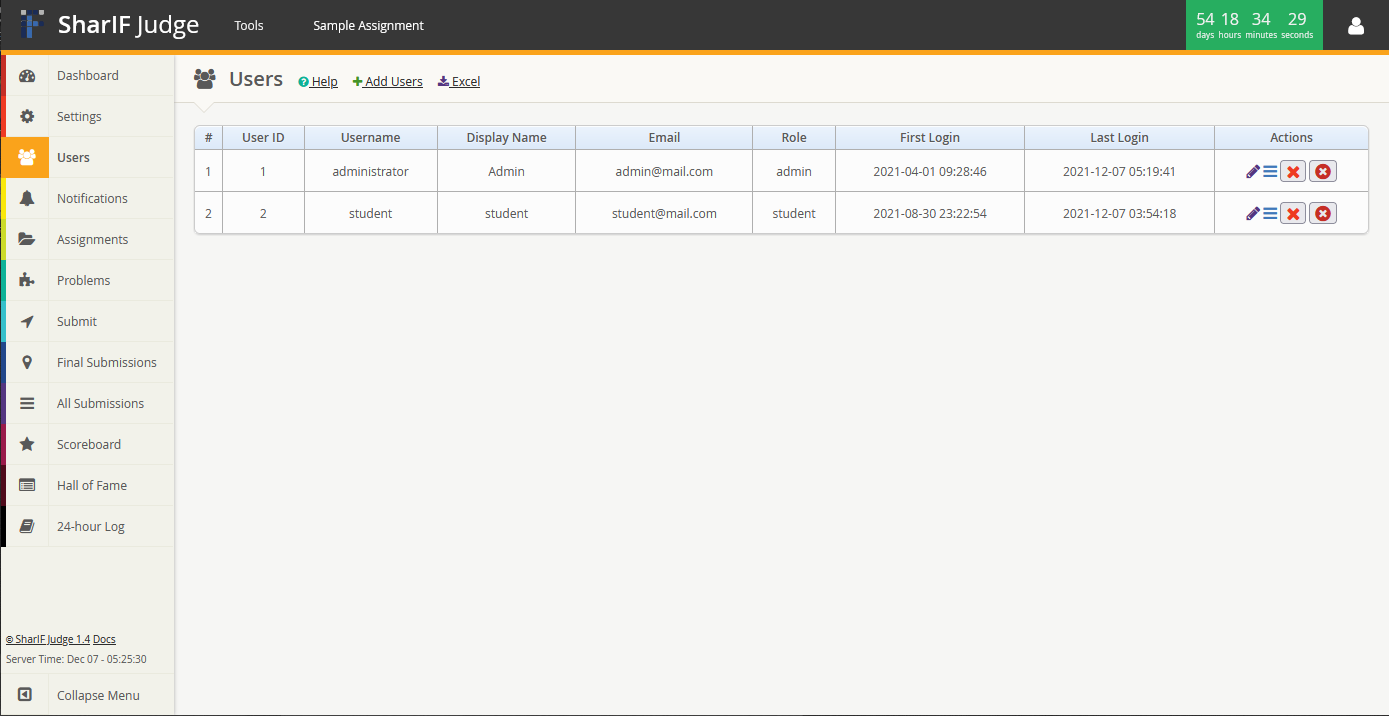
\includegraphics[scale=0.35]{Page/users.PNG}  
    	\caption{Halaman Users}
    	\label{fig:3:users} 
    \end{figure} 
    
    Gambar \ref{fig:3:users} menunjukkan halaman Users. Pada halaman ini terdapat daftar seluruh pengguna yang terdaftar pada SharIF Judge. Pengguna juga dapat membuat, mengubah, dan menghapus pengguna.
    
\subsubsection{Notifications}
    \begin{figure}[H]
    	\centering  
    	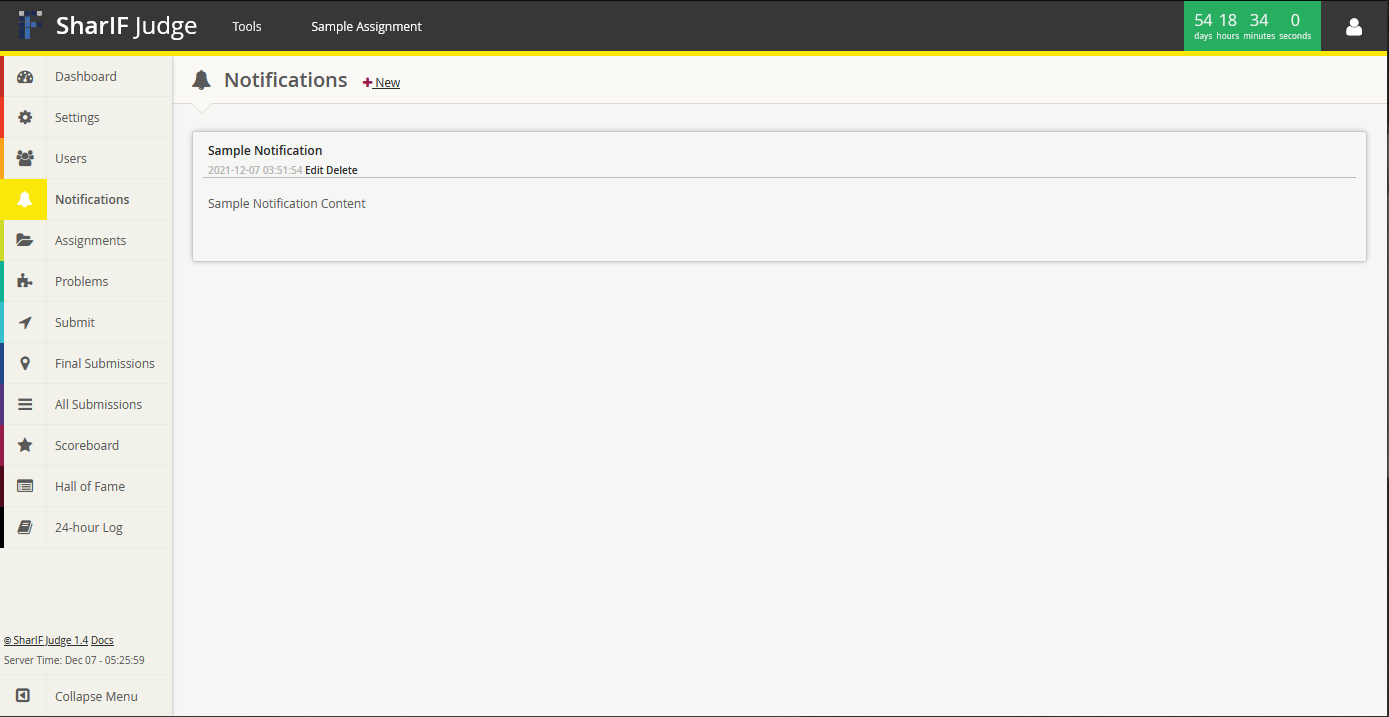
\includegraphics[scale=0.35]{Page/notifications.PNG}  
    	\caption{Halaman Notifications}
    	\label{fig:3:notifications} 
    \end{figure} 
    
    Gambar \ref{fig:3:notifications} menunjukkan halaman Notifications. Pada halaman ini terdapat daftar seluruh notifikasi. Pengguna juga dapat membuat, mengubah, dan menghapus notifikas.

\subsubsection{Assignments}
    \begin{figure}[H]
    	\centering  
    	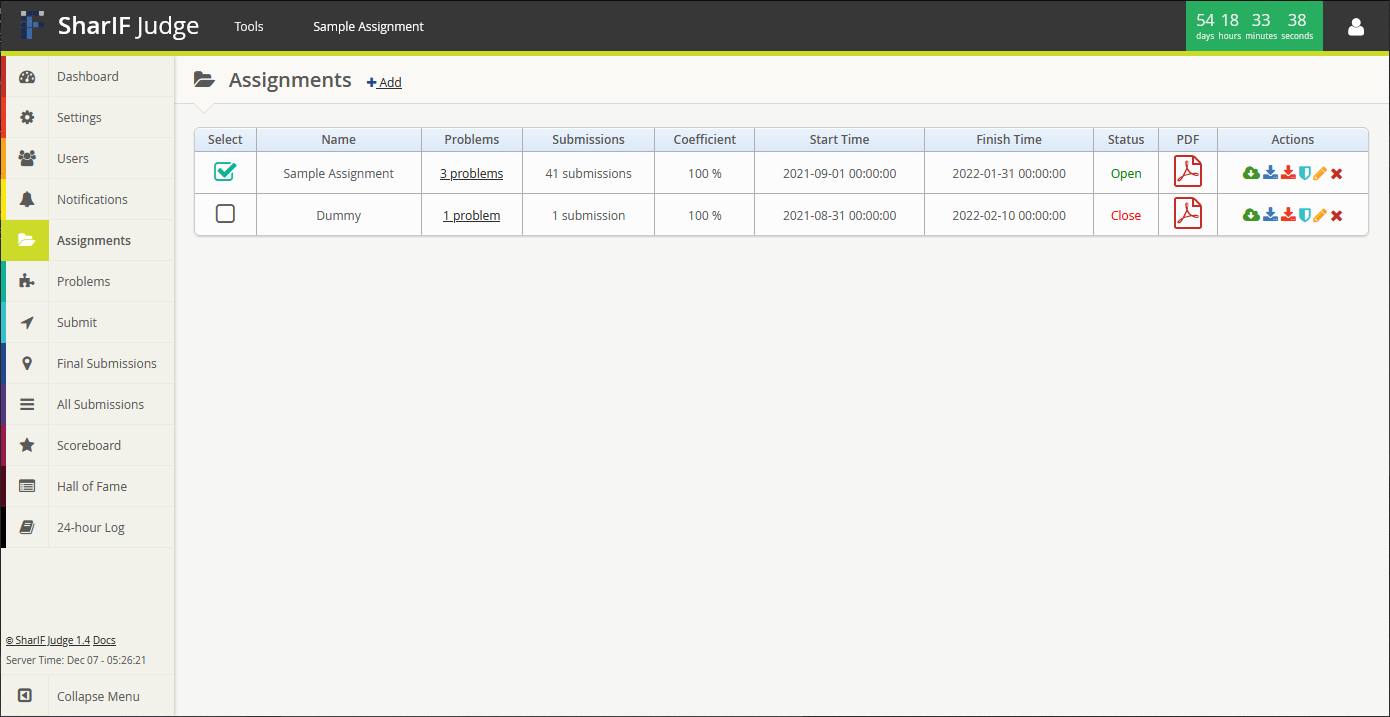
\includegraphics[scale=0.35]{Page/assignments.PNG}  
    	\caption{Halaman Assignments}
    	\label{fig:3:assignments} 
    \end{figure} 
    
    Gambar \ref{fig:3:assignments} menunjukkan halaman Assignments. Pada halaman ini terdapat daftar seluruh \textit{assignment}. Pengguna juga dapat membuat, mengubah, dan menghapus \textit{assignment}. Salah satu \textit{assignment} pada halaman ini harus dipilih untuk dapat menggunakan beberapa fitur lainnya pada SharIF Judge. Soal dalam bentuk PDF juga dapat diunduh melalui halaman ini. 
    
\subsubsection{Problems}
    \begin{figure}[H]
    	\centering  
    	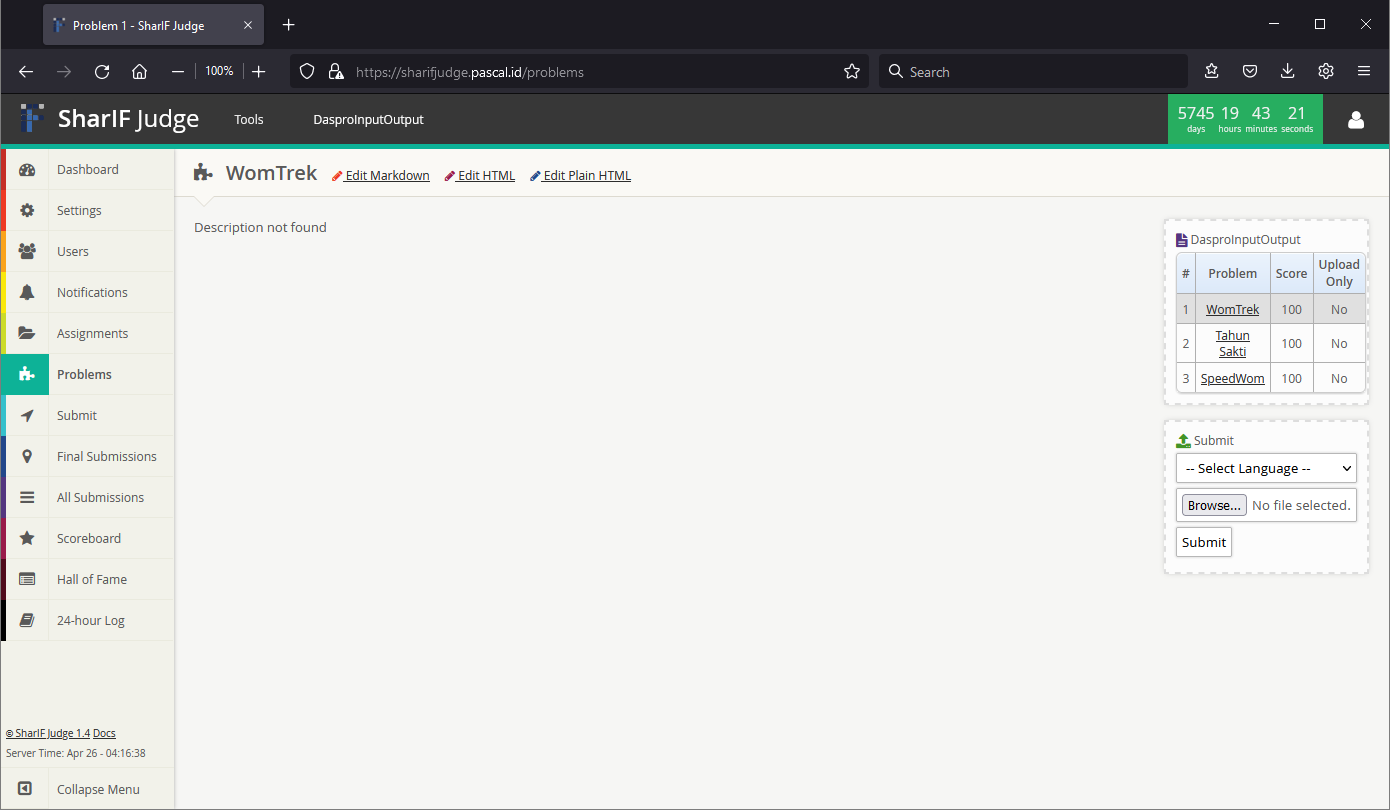
\includegraphics[scale=0.35]{Page/problems.PNG}  
    	\caption{Halaman Problems}
    	\label{fig:3:problems} 
    \end{figure} 
    
    Gambar \ref{fig:3:problems} menunjukkan halaman Problems. Pada halaman ini terdapat detil dari setiap \textit{problem} dari \textit{assignment} yang dipilih. Pengguna juga dapat mengunggah file untuk dikumpulkan sebagai \textit{submission} untuk \textit{problem} yang dipilih.
    
\subsubsection{Submit}
    \begin{figure}[H]
    	\centering  
    	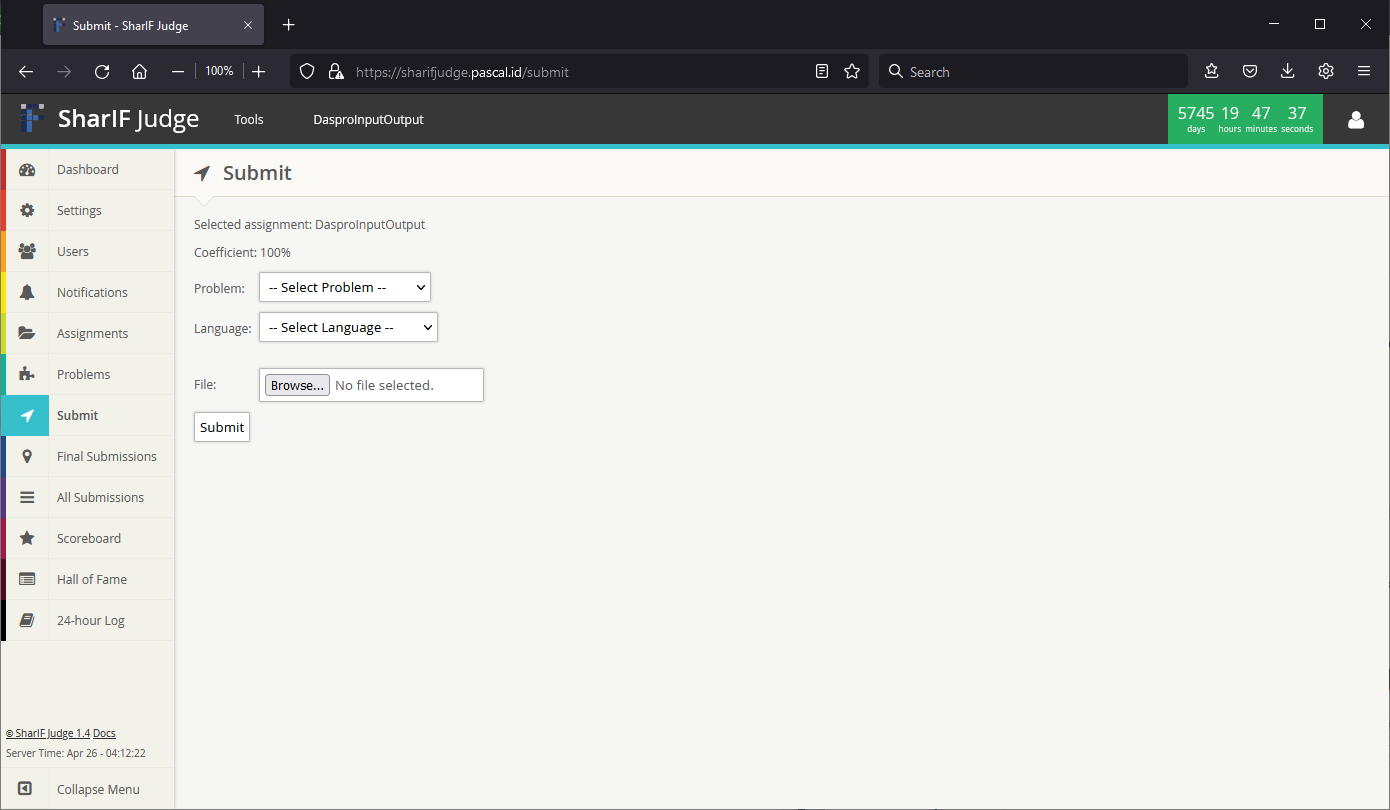
\includegraphics[scale=0.35]{Page/submit.PNG}  
    	\caption{Halaman Submit}
    	\label{fig:3:submit} 
    \end{figure} 
    
    Gambar \ref{fig:3:submit} menunjukkan halaman Submit. Pada halaman ini, pengguna dapat mengunggah file untuk dikumpulkan sebagai \textit{submission} dari \textit{problem} yang dipilih.

\subsubsection{Final Submissions}
    \begin{figure}[H]
    	\centering  
    	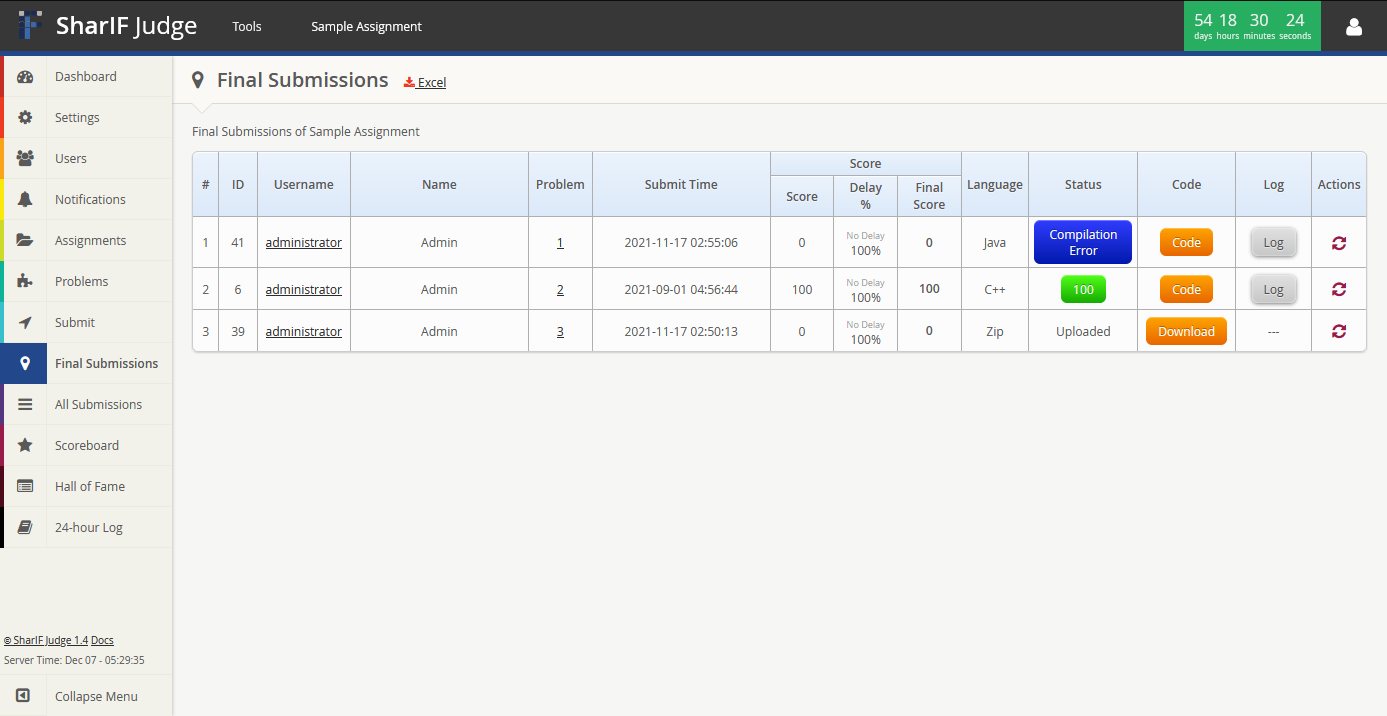
\includegraphics[scale=0.35]{Page/final_submissions.PNG}  
    	\caption{Halaman Final Submissions}
    	\label{fig:3:final_submissions} 
    \end{figure} 
    
    Gambar \ref{fig:3:final_submissions} menunjukkan halaman Final Submissions. Pada halaman ini, terdapat daftar seluruh \textit{final submission} untuk \textit{assignment} yang dipilih. Pengguna juga dapat melihat \textit{file} atau kode yang diunggah, dan nilai yang didapatkannya.
    
\subsubsection{All Submissions}
    \begin{figure}[H]
    	\centering  
    	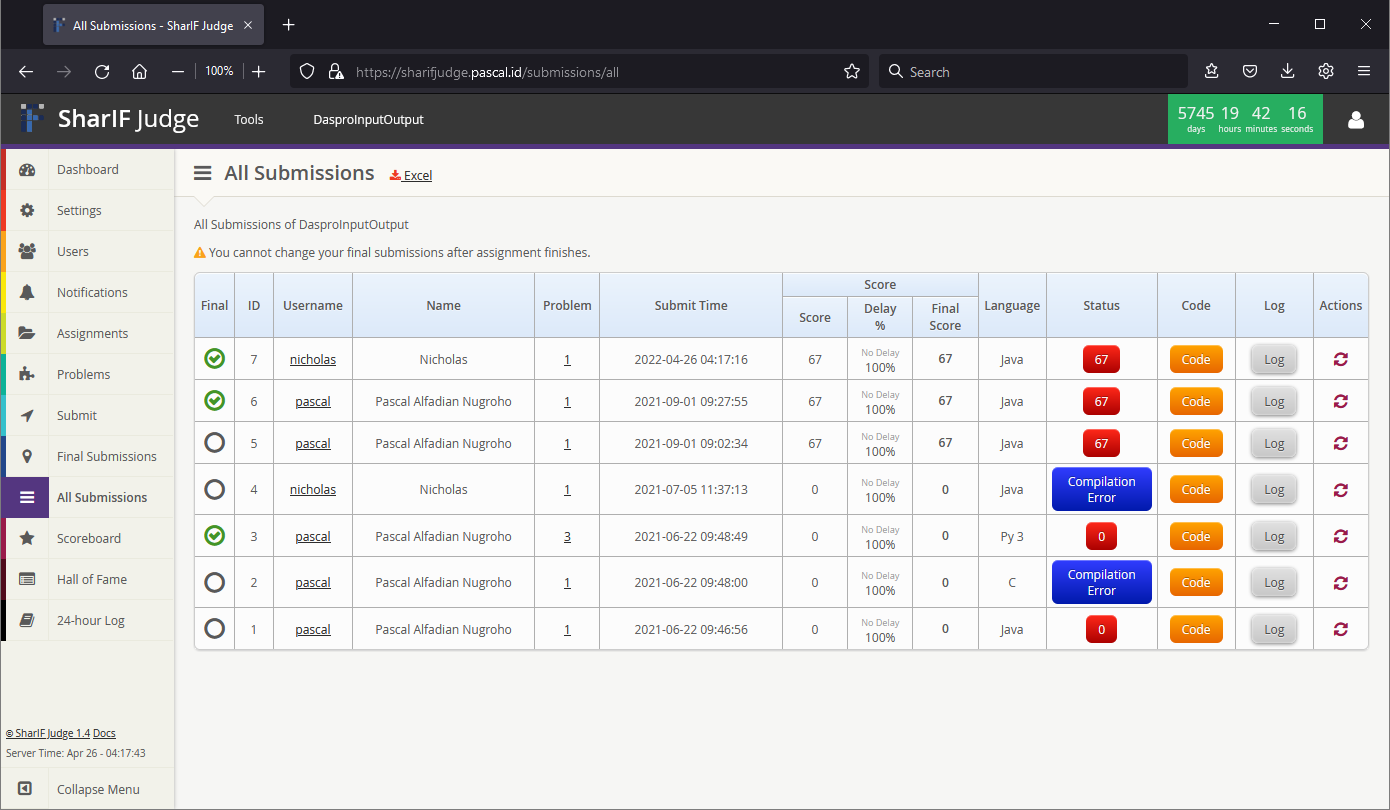
\includegraphics[scale=0.35]{Page/all_submissions.PNG}  
    	\caption{Halaman All Submissions}
    	\label{fig:3:all_submissions} 
    \end{figure} 
    
    Gambar \ref{fig:3:all_submissions} menunjukkan halaman All Submissions. Pada halaman ini, terdapat daftar seluruh \textit{submission} untuk \textit{assignment} yang dipilih. Pengguna juga dapat melihat \textit{file} atau kode yang diunggah, dan nilai yang didapatkannya. Untuk setiap \textit{problem}, sebuah \textit{submission} dapat dipilih sebagai \textit{final submission} melalui halaman ini.
    
\subsubsection{Scoreboard}
    \begin{figure}[H]
    	\centering  
    	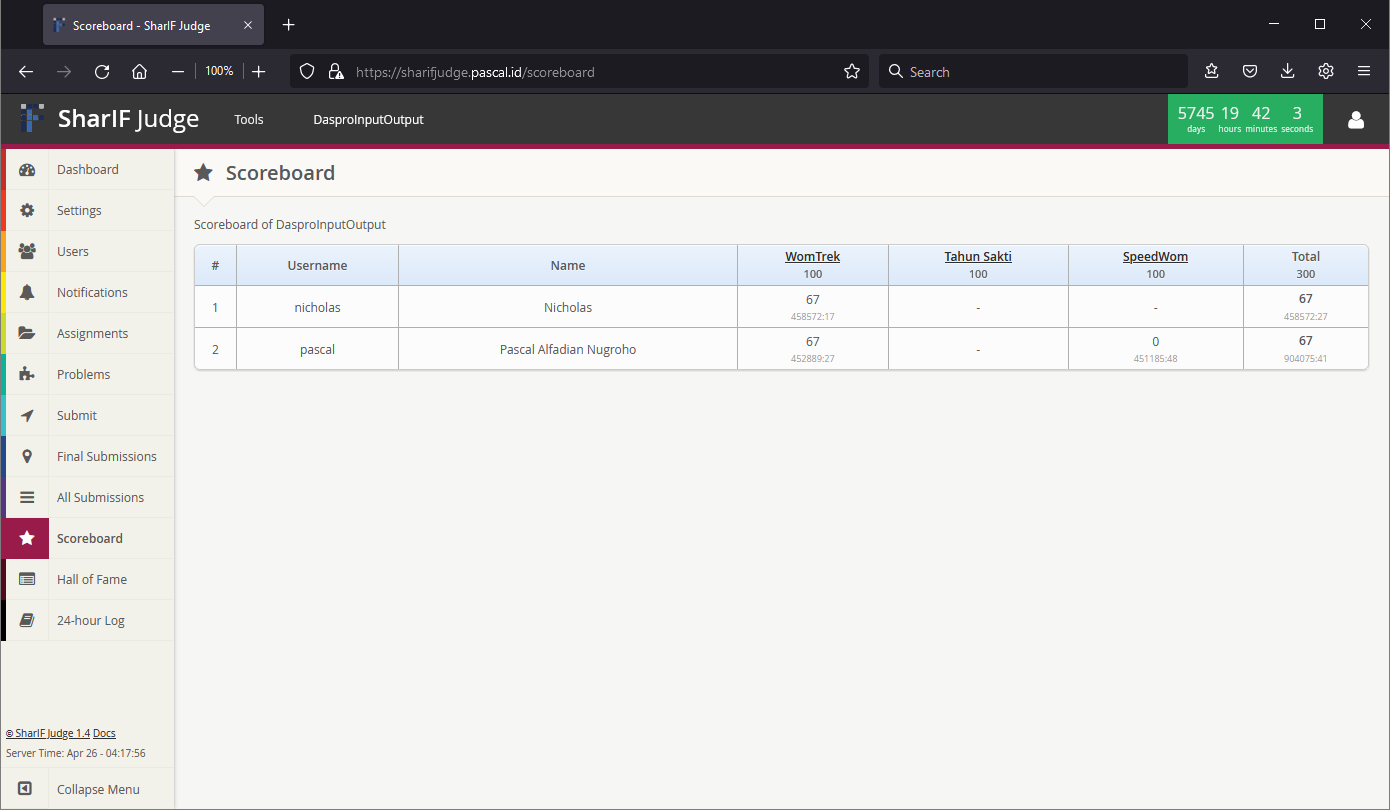
\includegraphics[scale=0.35]{Page/scoreboard.PNG}  
    	\caption{Halaman Scoreboard}
    	\label{fig:3:scoreboard} 
    \end{figure} 
    
    Gambar \ref{fig:3:scoreboard} menunjukkan halaman Scoreboard. Pada halaman ini, terdapat daftar nilai pengguna untuk setiap \textit{problem} pada \textit{assignment} yang dipilih.
    
\subsubsection{Hall of Fame}
    \begin{figure}[H]
    	\centering  
    	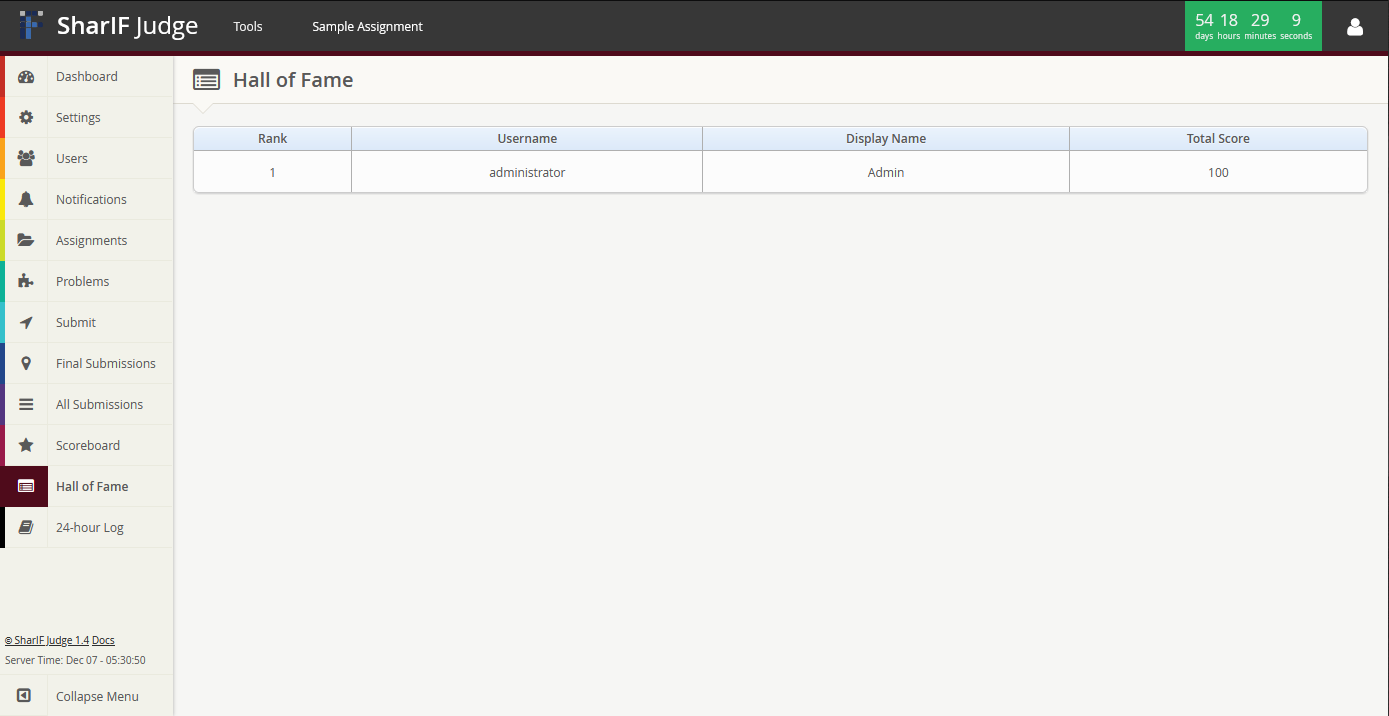
\includegraphics[scale=0.35]{Page/hall_of_fame.PNG}  
    	\caption{Halaman Hall of Fame}
    	\label{fig:3:hall_of_fame} 
    \end{figure} 
    
    Gambar \ref{fig:3:hall_of_fame} menunjukkan halaman Hall of Fame. Pada halaman ini, terdapat daftar pengguna secara berurutan berdasarkan total nilai yang didapatkannya dari seluruh \textit{assignment}.

\subsubsection{24-Hour Log}
    \begin{figure}[H]
    	\centering  
    	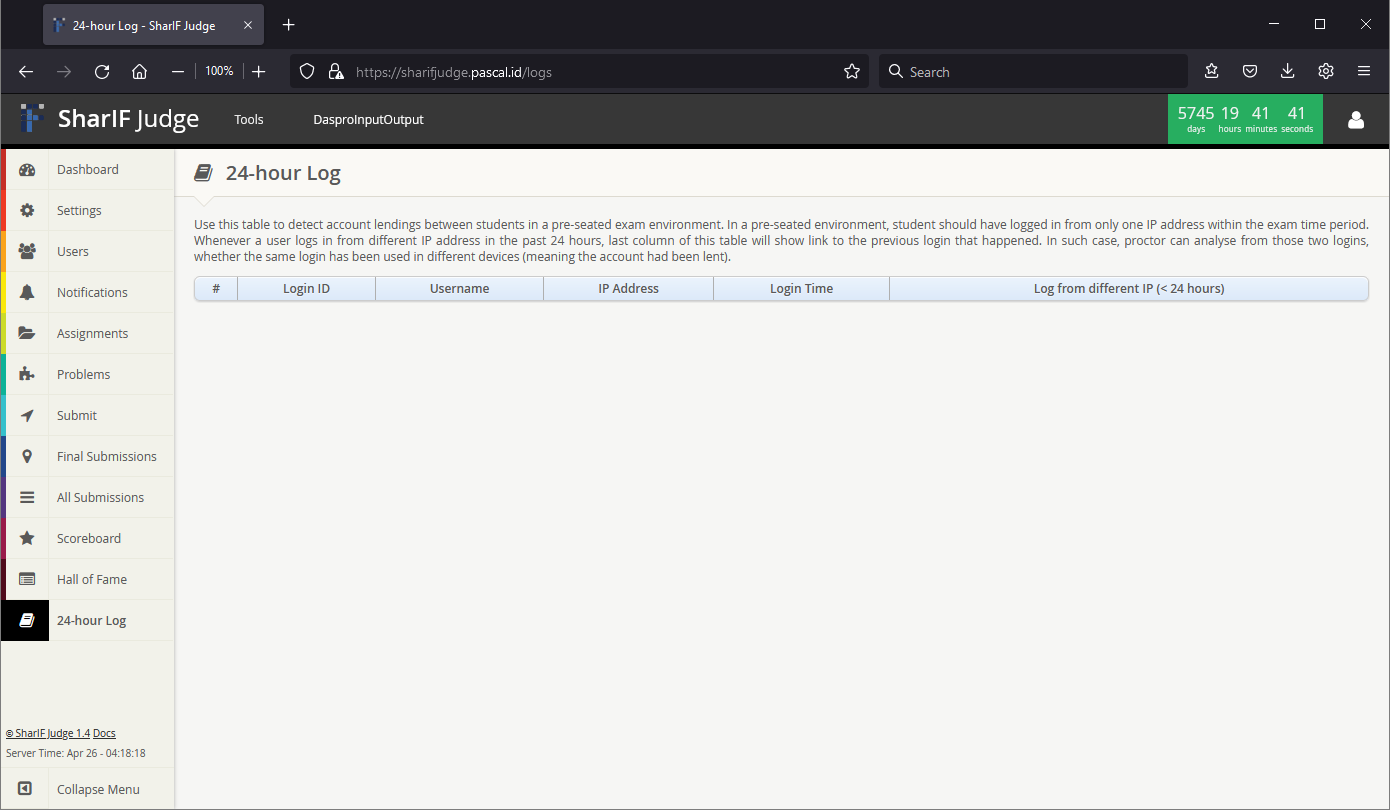
\includegraphics[scale=0.35]{Page/log.PNG}  
    	\caption{Halaman 24-Hour Log}
    	\label{fig:3:log} 
    \end{figure} 
    
    Gambar \ref{fig:3:log} menunjukkan halaman 24-Hour Log. Pada halaman ini, terdapat daftar yang mencatat bila akun yang sama melakukan \textit{login} dengan \textit{IP address} yang berbeda dalam jangka waktu 24 jam. Fitur ini digunakan untuk mendeteksi adanya peminjaman akun.

\subsection{Model, View, Controller}
\label{subs:3:mvc}
SharIF Judge menggunakan \textit{framework} CodeIgniter 3. Seperti yang dibahas pada bagian \ref{subs:2:cimvc}, \textit{framework} CodeIgniter menerapkan pola arsitektur MVC, dengan komponen-komponen \textit{model}, \textit{view}, dan \textit{controller}. Diagram kelas SharIF Judge dapat dilihat pada gambar \ref{fig:3:classdiagram}. Digunakan simbol komentar untuk komponen \textit{view} pada diagram ini, karena \textit{view} tidak berbentuk kelas.

    \begin{figure}[H]
    	\centering  
    	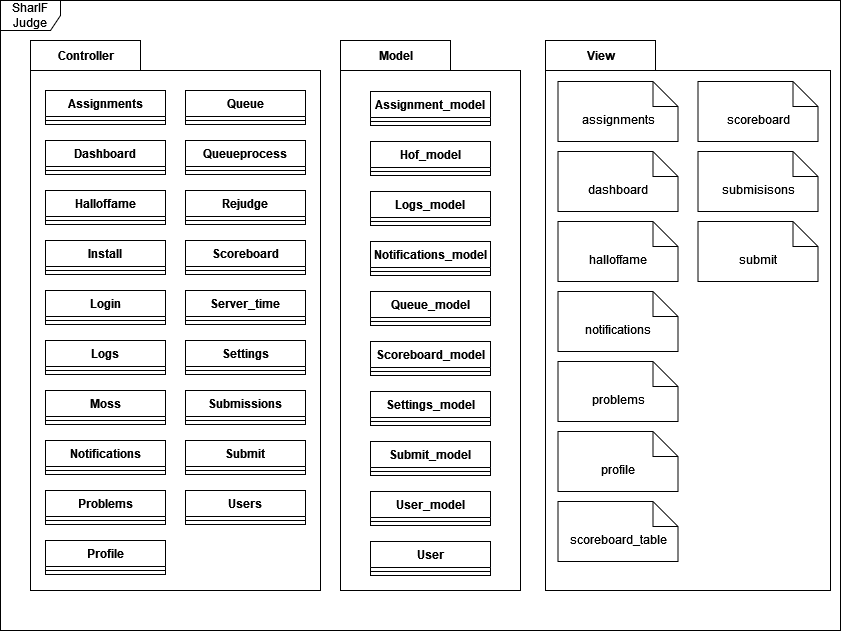
\includegraphics[scale=0.5]{Diagram/Class Diagram.PNG}  
    	\caption{Diagram kelas SharIF Judge}
    	\label{fig:3:classdiagram} 
    \end{figure} 


\subsubsection{Model}

Berikut ini adalah \textit{model} pada SharIF Judge:

\begin{itemize}
	\item \verb|Assignment_model| \\ Model untuk menangani tabel \verb|shj_assignments|. Fungsi yang dimiliki:
	\begin{itemize}
		\item \verb|add_assignment($id, $edit)|\\ Menambah atau memperbarui sebuah \textit{assignment}.
		\item \verb|delete_assignment($assignment_id)| \\ Menghapus sebuah \textit{assignment}.
		\item \verb|all_assignments()| \\ Mengambil seluruh \textit{assignment}.
		\item \verb|new_assignment_id()| \\ Menentukan \textit{integer} terkecil yang dapat digunakan sebagai id \textit{assignment} baru.
		\item \verb|all_problems($assignment_id)| \\ Mengambil seluruh \textit{problem} dari \textit{assignment}.
		\item \verb|problem_info($assignment_id, $problem_id)| \\ Mengambil sebuah \textit{problem}.
		\item \verb|assignment_info($assignment_id)| \\ Mengambil sebuah \textit{assignment}.
		\item \verb|is_participant($participants, $username)| \\ Mengembalikan \verb|TRUE| jika \verb|$username| terdapat dalam \verb|$participants|.
		\item \verb|increase_total_submits($assignment_id)| \\ Meningkatkan jumlah total \textit{submit} sebuah \textit{assignment} sebanyak satu.
		\item \verb|set_moss_time($assignment_id)| \\ Memperbarui "\textit{Moss Update Time}" untuk sebuah assignment.
		\item \verb|get_moss_time($assignment_id)| \\ Mengambil "\textit{Moss Update Time}" untuk sebuah assignment.
		\item \verb|save_problem_description($assignment_id, $problem_id, $text, $type)| \\ Menambah atau memperbarui deskripsi sebuah \textit{problem}.
		\item \verb|_update_coefficients($a_id, $extra_time, $finish_time, $new_late_rule)| \\ Memperbarui koefisien seluruh \textit{submission} pada sebuah \textit{assignment}.
	\end{itemize}
	
	\item \verb|Hof_model| \\ Model untuk menangani informasi \textit{hall of fame}. Fungsi yang dimiliki:
	\begin{itemize}
	    \item \verb|get_all_final_submission()| \\ Mengambil seluruh \textit{final submission}.
	    \item \verb|get_all_user_assignments($username)| \\ Mengambil seluruh \textit{assignment} dan \textit{problem} untuk \textit{user} tertentu.
	\end{itemize}
	
	\item \verb|Logs_model| \\ Model untuk menangani tabel \verb|shj_logins|. Fungsi yang dimiliki:
	\begin{itemize}
	    \item \verb|insert_to_logs($username, $ip_adrress)| \\ Menambah sebuah catatan \textit{login} dan menghapus catatan yang sudah melebihi 24 jam.
	    \item \verb|get_all_logs()| \\ Mengambil seluruh catatan \textit{login}.
	\end{itemize}
	
	\item \verb|Notifications_model| \\ Model untuk menangani tabel \verb|shj_notifications|. Fungsi yang dimiliki:
	\begin{itemize}
	    \item \verb|get_all_notifications()| \\ Mengambil seluruh notifikasi.
	    \item \verb|get_latest_notifications()| \\ Mengambil 10 notifikasi terbaru.
	    \item \verb|add_notification($title, $text)| \\ Menambah notifikasi baru.
	    \item \verb|update_notification($id, $title, $text)| \\ Memperbarui sebuah notifikasi. 
	    \item \verb|delete_notification($id)| \\ Menghapus sebuah notifikasi.
	    \item \verb|get_notification($notif_id)| \\ Mengambil sebuah notifikasi.
	    \item \verb|have_new_notification($time)| \\ Mengembalikan \verb|TRUE| jika terdapat notifikasi setelah \verb|$time|.
	\end{itemize}
	
	\item \verb|Queue_model| \\ Model untuk menangani tabel \verb|shj_queue|. Fungsi yang dimiliki:
	\begin{itemize}
	    \item \verb|in_queue($username, $assignment, $problem)| \\ Mengembalikan \verb|TRUE| jika sebuah \textit{submission} sudah berada dalam antrean.
	    \item \verb|get_queue()| \\ Mengambil seluruh antrean.
	    \item \verb|empty_queue()| \\ Mengosongkan antrean.
	    \item \verb|add_to_queue($submit_info)| \\ Menambahkan sebuah \textit{submission} ke dalam antrean.
	    \item \verb|rejudge($assignment_id, $problem_id)| \\ Menambahkan seluruh \textit{submission} dari sebuah \textit{problem} ke dalam antrean untuk dinilai ulang.
	    \item \verb|rejudge_single($submission)| \\  Menambahkan sebuah \textit{submission} ke dalam antrean untuk dinilai ulang.
	    \item \verb|get_first_item()| \\ Mengambil baris pertama dari antrean.
	    \item \verb|remove_item($username, $assignment, $problem, $submit_id)| \\ Menghapus sebuah baris dari antrean.
	    \item \verb|save_judge_result_in_db ($submission, $type)| \\ Menyimpan hasil penilaian ke dalam \textit{database}.
	\end{itemize}
	
	\item \verb|Scoreboard_model| \\ Model untuk menangani tabel \verb|shj_scoreboard|. Fungsi yang dimiliki:
	\begin{itemize}
	    \item \verb|_generate_scoreboard($assignment_id)| \\ Membuat \textit{scoreboard} untuk sebuah \textit{assignment}.
	    \item \verb|update_scoreboards()| \\ Memperbarui \textit{scoreboard} untuk seluruh \textit{assignment}.
	    \item \verb|update_scoreboard($assignment_id)| \\ Memperbarui \textit{scoreboard} untuk sebuah \textit{assignment}.
	    \item \verb|get_scoreboard($assignment_id)| \\ Mengambil \textit{scoreboard} untuk sebuah \textit{assignment}.
	\end{itemize}
	
	\item \verb|Settings_model| \\ Model untuk menangani tabel \verb|shj_settings|. Fungsi yang dimiliki:
	\begin{itemize}
	    \item \verb|get_setting($key)| \\ Mengambil sebuah pengaturan.
	    \item \verb|set_setting($key, $value)| \\ Memperbarui sebuah pengaturan.
	    \item \verb|get_all_settings()| \\ Mengambil seluruh pengaturan.
	    \item \verb|set_settings($settings)| \\ Memperbarui beberapa pengaturan.
	\end{itemize}
	
	\item \verb|Submit_model| \\ Model untuk menangani tabel \verb|shj_submissions|. Fungsi yang dimiliki:
	\begin{itemize}
	    \item \verb|get_submission($uname, $assignment, $problem, $submit_id)| \\ Mengambil sebuah \textit{submission}.
	    \item \verb|get_final_submissions($a_id, $u_lv, $uname, $p_num, $f_user, $f_prblm)| \\ Mengambil seluruh \textit{final submission} untuk sebuah \textit{assignment}.
	    \item \verb|get_all_submissions($a_id, $u_lv, $uname, $p_num, $f_user, $f_prblm)| \\ Mengambil seluruh \textit{submission} untuk sebuah \textit{assignment}.
	    \item \verb|count_final_submissions($a_id, $u_lv, $uname, $f_user, $f_prblm)| \\ Menghitung jumlah \textit{final submission} dari \textit{user} tertentu.
	    \item \verb|count_all_submissions($a_id, $u_lv, $uname, $f_user, $f_prblm)| \\ Menghitung jumlah \textit{submission} dari \textit{user} tertentu.
	    \item \verb|set_final_submission($uname, $assignment, $problem, $submit_id)| \\ Memperbarui sebuah \textit{submission} menjadi \textit{final}.
	    \item \verb|add_upload_only($submit_info)| \\ Menambahkan hasil dari \textit{submission} \textit{upload only} ke dalam \textit{database}.
	\end{itemize}
	
	\item \verb|User| \\ Model untuk menangani informasi preferensi setiap \textit{user}. Fungsi yang dimiliki:
	\begin{itemize}
	    \item \verb|select_assignment($assignment_id)| \\ Menetapkan \textit{assignment} yang dipilih.
	    \item \verb|save_widget_positions($positions)| \\ Memperbarui posisi \textit{widget}.
	    \item \verb|get_widget_positions()| \\ Mengambil posisi \textit{widget}.
	\end{itemize}
	
	\item \verb|User_model| \\ Model untuk menangani tabel \verb|shj_users|. Fungsi yang dimiliki:
	\begin{itemize}
	    \item \verb|have_user($username)| \\ Mengembalikan \verb|TRUE| jika terdapat \textit{user} dengan nama \verb|$username|.
	    \item \verb|user_id_to_username($user_id)| \\ Mengembalikan \verb|username| dari \textit{user} dengan \verb|id| tertentu.
	    \item \verb|username_to_user_id($username)| \\ Mengembalikan \verb|id| dari \textit{user} dengan \verb|username| tertentu.
	    \item \verb|have_email($email, $username)| \\ Mengembalikan \verb|TRUE| jika terdapat \textit{user} selain \verb|$username| dengan email \verb|$email|.
	    \item \verb|add_user($username, $email, $display_name, $password, $role)| \\ Menambahkan sebuah \textit{user} baru.
	    \item \verb|add_users($text, $send_mail, $delay)| \\ Menambahkan beberapa \textit{user} baru.
	    \item \verb|delete_user($user_id)| \\ Menghapus sebuah \textit{user}.
	    \item \verb|delete_submissions($user_id)| \\ Menghapus seluruh \textit{submission} dari sebuah \textit{user}.
	    \item \verb|validate_user($username, $password)| \\ Mengembalikan \verb|TRUE| jika \verb|$username| dan \verb|$password| valid untuk login.
	    \item \verb|selected_assignment($username)| \\ Mengembalikan \textit{assignment} yang dipilih sebuah \textit{user}.
	    \item \verb|get_names()| \\  Mengembalikan nama dari \textit{user}.
	    \item \verb|update_profile($user_id)| \\ Memperbarui sebuah \textit{user}.
	    \item \verb|send_password_reset_mail($email)| \\ Mengirim \textit{email} untuk \textit{reset password}.
	    \item \verb|passchange_is_valid($passchange_key)| \\ Mengembalikan \verb|TRUE| jika kunci untuk \textit{reset password} valid.
	    \item \verb|reset_password($passchange_key, $newpassword)| \\ Memperbarui \textit{password} menjadi kunci \textit{reset password}.
	    \item \verb|get_all_users()| \\ Mengambil seluruh \textit{user}.
	    \item \verb|get_user($user_id)| \\ Mengambil sebuah \textit{user}.
	    \item \verb|update_login_time($username)| \\ Memperbarui catatan \textit{login} sebuah \textit{user}.
	\end{itemize}
\end{itemize}

\subsubsection{View}

\textit{View} pada SharIF Judge terbagi menjadi beberapa folder:

\begin{itemize}
    \begin{figure}[H]
    	\centering
    	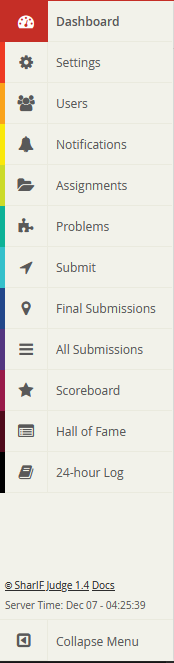
\includegraphics[scale=0.35]{View/sidebar}  
    	\caption{Tampilan \textit{top bar} pada \texttt{top\_bar.twig} dan \textit{side bar} pada \texttt{side\_bar.twig}}
    	\label{fig:3:viewsidebar} 
    \end{figure} 
    \item \verb|templates| \\ Menyimpan komponen-komponen dasar halaman. Pada gambar \ref{fig:3:viewsidebar}, area yang ditandai dengan kotak merah adalah komponen dasar \textit{top bar} dan \textit{side bar}.
    
    \begin{figure}[H]
    	\centering  
    	\includegraphics[scale=0.35]{View/dashboard}  
    	\caption{Tampilan Dashboard pada \texttt{dashboard.twig}}
    	\label{fig:3:viewsubmit} 
    \end{figure} 
    \item \verb|pages| \\ Menyimpan komponen utama halaman. Pada gambar \ref{fig:3:viewsubmit}, area yang ditandai dengan kotak merah adalah komponen utama halaman Dashboard.
    
    \begin{figure}[H]
    	\centering  
    	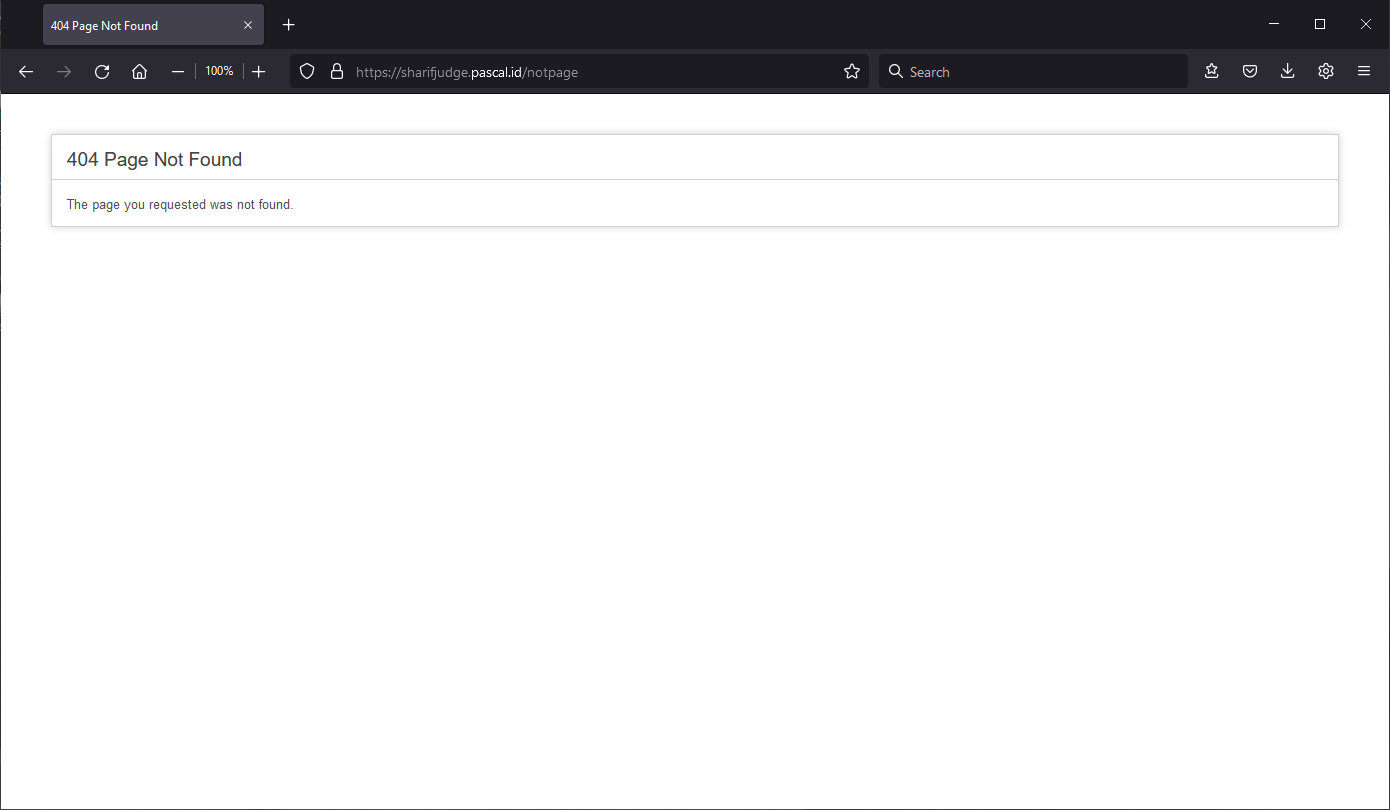
\includegraphics[scale=0.35]{View/404}  
    	\caption{Tampilan halaman \textit{error} pada \texttt{error\_404.php}}
    	\label{fig:3:view404} 
    \end{figure} 
	\item \verb|errors| \\ Menyimpan tampilan halaman error. Gambar \ref{fig:3:view404} adalah contoh halaman error 404.
\end{itemize}

\subsubsection{Controller}

Berikut ini adalah \textit{controller} pada SharIF Judge:

\begin{itemize}
	\item \verb|Assignments| \\ Controller untuk menangani \textit{assignments}. Fungsi yang dimiliki:
	\begin{itemize}
		\item \verb|select()| \\ Memilih \textit{assignment} yang sedang ditampilkan.
		\item \verb|pdf($assignment_id, $problem_id)| \\ Mengunduh \textit{file} PDF dari sebuah \textit{assignment}.
		\item \verb|downloadtestsdesc($assignment_id)| \\ Mengunduh \textit{file} \textit{test case} dari sebuah \textit{assignment}.
		\item \verb|download_submissions($type, $assignment_id)| \\ Mengunduh seluruh \textit{file} \textit{final submission} dari sebuah \textit{assignment}.
		\item \verb|delete($assignment_id)| \\ Menghapus sebuah \textit{assignment}.
		\item \verb|add()| \\ Menambah atau memperbarui \textit{assignment}.
		\item \verb|edit($assignment_id)| \\ Memperbarui \textit{assignment}.
	\end{itemize}
	
	\item \verb|Dashboard| \\Controller untuk menangani halaman \textit{Dashboard}. Fungsi yang dimiliki:
	\begin{itemize}
		\item \verb|widget_positions()| \\ Menyimpan posisi \textit{widget} dari \textit{user}.
	\end{itemize}
	
	\item \verb|Halloffame| \\ Controller untuk menangani halaman \textit{Hall of Fame} . Fungsi yang dimiliki:
	\begin{itemize}
		\item \verb|hof_details()| \\ Mengambil data yang diperlukan untuk \textit{hall of fame}.
	\end{itemize}
	
	\item \verb|Install| \\ Controller untuk menangani instalasi SharIF Judge.
	
	\item \verb|Login| \\ Controller untuk menangani halaman-halaman \textit{login}. Fungsi yang dimiliki:
	\begin{itemize}
		\item \verb|register()| \\ Registrasi \textit{user} baru dan menampilkan halaman \textit{register}.
		\item \verb|logout()| \\ \textit{Log out} user saat ini dan mengalihkan ke halaman \textit{login}.
		\item \verb|lost()| \\ Menangani email dan menampilkan halaman untuk meminta \textit{reset password}.
		\item \verb|reset($passchange_key)| \\ Memproses dan menampilkan halaman untuk ubah \textit{reset password}.
	\end{itemize}
	
	\item \verb|Logs| \\ Controller untuk menangani halaman \textit{24-hour Log}.
	\begin{itemize}
        \item \verb|index()| Mengambil data yang diperlukan dan menampilkan halaman \textit{24-hour Log}.
	\end{itemize}
	
	\item \verb|Moss| \\ Controller untuk menangani halaman \textit{Detect Similar Codes} . Fungsi yang dimiliki:
	\begin{itemize}
		\item \verb|update($assignment_id)| \\ Memperbarui informasi pada halaman \textit{Detect Similar Codes}.
		\item \verb|_detect($assignment_id)| \\ Menjalankan Moss untuk mendeteksi kesamaan kode.
	\end{itemize}
	
	\item \verb|Notifications| \\ Controller untuk menangani halaman \textit{Notifications}. Fungsi yang dimiliki:
	\begin{itemize}
		\item \verb|add()| \\ Menambahkan notifikasi baru dan menampilkan halaman \textit{New Notification}.
		\item \verb|edit($notif_id)| \\ Memperbarui sebuah notifikasi.
		\item \verb|delete()| \\ Menghapus sebuah notifikasi.
		\item \verb|check()| \\ Memeriksa adanya notifikasi baru.
	\end{itemize}
	
	\item \verb|Problems| \\ Controller untuk menangani halaman \textit{Problems}. Fungsi yang dimiliki:
	\begin{itemize}
		\item \verb|index($assignment_id, $problem_id = 1)| \\ Mengambil data yang diperlukan dan menampilkan halaman \textit{Problems}.
		\item \verb|edit($type = 'md', $assignment_id, $problem_id = 1)| \\ Memperbarui deskripsi \textit{problem} dan menampilkan halaman \textit{Edit Problem Description}.
	\end{itemize}
	
	\item \verb|Profile| \\ Controller untuk menangani halaman \textit{Profile}. Fungsi yang dimiliki:
	\begin{itemize}
		\item \verb|index($user_id)| \\ Mengambil data yang diperlukan dan menampilkan halaman \textit{Profile}.
		\item \verb|_password_check($str)| \\ Memeriksa apakah \textit{password} sesuai dengan syarat.
		\item \verb|_password_again_check($str)| \\ Memeriksa apakah \textit{password again} sama dengan \textit{password} yang dimasukkan.
		\item \verb|_email_check($email)| \\ Memeriksa apakah terdapat user dengan alamat email tertentu.
		\item \verb|_role_check($role)| \\ Memeriksa \textit{role} yang dimiliki \textit{user}.
	\end{itemize}
	
	\item \verb|Queue| \\ Controller untuk menangani halaman \textit{Queue}. Fungsi yang dimiliki:
	\begin{itemize}
        \item \verb|index()| \\ Mengambil data yang diperlukan dan menampilkan halaman \textit{Queue}.
        \item \verb|pause()| \\ Memberhentikan antrean.
        \item \verb|resume()| \\ Melanjutkan antrean.
        \item \verb|empty_queue()| \\ Mengosongkan antrean.
	\end{itemize}
	
	\item \verb|Queueprocess| \\Controller untuk menangani proses penilaian kode. Fungsi yang dimiliki:
	\begin{itemize}
        \item \verb|run()| \\ Menilai kode satu per satu dari antrean.
	\end{itemize}
	
	\item \verb|Rejudge| \\ Controller untuk menangani halaman \textit{Rejudge}. Fungsi yang dimiliki:
	\begin{itemize}
        \item \verb|index()| \\ Mengambil data yang diperlukan dan menampilkan halaman \textit{Rejudge}.
        \item \verb|rejudge_single()| \\ Melakukan penilaian ulang untuk sebuah \textit{submission}.
	\end{itemize}
	
	\item \verb|Server_time| \\ Controller untuk menangani sinkronisasi waktu server. Fungsi yang dimiliki:
	\begin{itemize}
        \item \verb|index()| \\ Mengembalikan waktu server.
	\end{itemize}
	
	\item \verb|Submissions| \\ Controller untuk menangani unduh \textit{submissions} menjadi file Excel. Fungsi yang dimiliki:
	\begin{itemize}
        \item \verb|_download_excel($view)| \\ Menggunakan \textit{library} PHPExcel untuk membuat file excel.
        \item \verb|final_excel()| \\ Mengunduh data \textit{final submissions} sebagai file excel.
        \item \verb|all_excel()| \\ Mengunduh data \textit{final submissions} sebagai file excel.
        \item \verb|the_final()| \\ Mengambil dan menampilkan data \textit{final submissions} yang akan diunduh.
        \item \verb|all()| \\ Mengambil dan menampilkan data \textit{submissions} yang akan diunduh.
        \item \verb|select()| \\ Memilih \textit{final submission}.
        \item \verb|view_code()| \\ Menampilkan kode, \textit{result}, atau \textit{log} dari \textit{submission}.
        \item \verb|download_file()| \\ Mengunduh file excel.
	\end{itemize}
	
	\item \verb|Submit| \\ Controller untuk menangani \textit{submissions}. Fungsi yang dimiliki:
	\begin{itemize}
        \item \verb|_language_to_type($language)| \\ Mengembalikan kode singkatan dari bahasa pemrograman.
        \item \verb|_match($type, $extension)| \\ Memeriksa apakah bahasa pemrograman dan tipe file sesuai.
        \item \verb|_check_language($str)| \\ Memeriksa apakah bahasa pemrograman yang dipilih valid.
        \item \verb|index()| \\ Mengambil data yang diperlukan dan menampilkan halaman \textit{Submit}.
        \item \verb|_upload()| \\ Menyimpan file yang diunggah dan menambahkannya ke dalam antrean.
	\end{itemize}
	
	\item \verb|Users| \\ Controller untuk menangani halaman \textit{Users}. Fungsi yang dimiliki:
	\begin{itemize}
        \item \verb|index()| \\ Mengambil data yang diperlukan dan menampilkan halaman \textit{Users}.
        \item \verb|add()| \\ Menambah \textit{user} baru dan menampilkan halaman \textit{Add Users}.
        \item \verb|delete()| \\ Menghapus \textit{user}.
        \item \verb|delete_submissions()| \\ Menghapus seluruh \textit{submission} dari sebuah \textit{user}.
         \item \verb|list_excel()| \\ Menggunakan \textit{library} PHPExcel untuk membuat file excel dari \textit{list user}.
	\end{itemize}
\end{itemize}

\subsection{Penyimpanan Kode}
\label{subsec:3:simpan}

Pada SharIF Judge, seluruh kode yang diunggah pengguna disimpan dalam \textit{folder} \verb|assignments|. Lokasi \textit{folder} \verb|assignments| dapat diubah pada halaman Settings. Kode yang diunggah disimpan pada \textit{folder} \verb|assignments| dengan format alamat \lstinline{assignment_<assignment_id>/p_<problem_id>/<nama_pengguna>/<nama_file_yang_diupload>-<submit_id>.<ekstensi_file>}, dengan penjelasan sebagai berikut:
\begin{itemize}
    \item \verb|<assignment_id>| \\ \verb|id| dari \textit{assignment} yang dipilih.
    \item \verb|<problem_id>| \\ \verb|id| dari \textit{problem} yang dipilih.
    \item \verb|<nama_pengguna>| \\ Nama pengguna yang mengunggah \textit{file}.
    \item \verb|<nama_file_yang_diupload>| \\ Nama \textit{file} yang diunggah.
    \item \verb|<submit_id>| \\ \verb|id| dari \textit{submission} yang diunggah.
    \item \verb|<ekstensi_file>| \\ Ekstensi \textit{file} yang diunggah.
\end{itemize}

Sebagai contoh, seorang pengguna bernama \verb|user| mengunggah sebuah \textit{file} bernama \verb|mycode.java| untuk \textit{problem} ke-3 pada \textit{assignment} dengan id 5. \textit{Submission} pengguna ini adalah \textit{submission} ke-20 untuk \textit{problem} tersebut, sehingga \verb|submit_id| adalah 20. Maka alamat penyimpanan untuk contoh ini adalah \verb|assignment_5/p_3/user/mycode-20.java|.


\subsection{Antrean Penilaian Kode}
\label{subsec:3:antrean} 
Pada SharIF Judge, seluruh kode yang dikumpulkan pengguna akan dijalankan satu per satu dalam antrean untuk dinilai. Tahap-tahap yang dilalui sebuah kode hingga penilaian selesai adalah sebagai berikut:

\begin{enumerate}
    \item \textit{Controller} \verb|Submit| menyimpan \textit{file} kode pada folder sesuai dengan penjelasan pada bab \ref{subsec:3:simpan}.
    \item \textit{Model} \verb|Queue_model| menyimpan \textit{submission} pada basis data \verb|shj_submissions|, lalu dimasukkan dalam antrean pada basis data \verb|shj_queue|.
    \item \textit{Controller} \verb|Submit| memanggil fungsi \verb|process_the_queue()| yang menjalankan fungsi \verb|run()| pada \textit{controller} \verb|Queueprocess|.
    \item \textit{Controller} \verb|Queueprocess| membaca setiap baris basis data \verb|shj_queue| satu per satu untuk dinilai dengan menjalankan \verb|tester.sh|.
    \item \verb|tester.sh| mengompilasi kode, menjalankan kode dengan tes kasus, menilai hasilnya dengan kunci jawaban, lalu mengembalikan hasil penilaian.
    \item \textit{Controller} \verb|Queueprocess| menyimpan nilai kembalian pada basis data \verb|shj_submissions| dan menghapus baris dari basis data \verb|shj_queue|.
\end{enumerate}

\section{Analisis Sistem Usulan}
\label{sec:3:analisisusulan} 
Agar SharIF Judge dapat menjadi sebuah IDE, SharIF Judge harus mampu untuk memfasilitasi seluruh proses pembuatan kode. Pada gambar \ref{fig:3:usecase}, terdapat Use Case Diagram sebagai tambahan dari diagram pada gambar \ref{fig:3:usecased} untuk fitur yang akan ditambahkan. Seluruh fitur yang akan ditambahkan dapat digunakan oleh setiap \textit{role} pengguna, yaitu \textit{Admin}, \textit{Head Instructor}, \textit{Instructor}, \textit{Student}.
   
    \begin{figure}[H]
    	\centering  
    	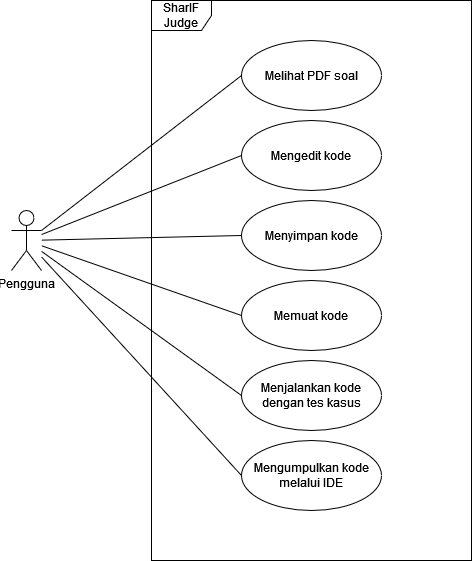
\includegraphics[scale=0.5]{Diagram/Use Case Usulan.PNG}  
    	\caption{Use Case Diagram Fitur Usulan}
    	\label{fig:3:usecase} 
    \end{figure} 

\pagebreak
Berikut ini merupakan skenario untuk masing-masing fitur yang akan ditambahkan pada SharIF Judge:

\begin{itemize}

    \item Melihat soal \\ Akan ditambahkan fitur untuk menampilkan soal PDF di halaman submit untuk \textit{assignment} yang dipilih, sehingga pengguna dapat melihat soal secara langsung pada SharIF Judge tanpa perlu mengunduhnya terlebih dahulu.
        \begin{itemize}
            \item Aktor: Pengguna
            \item Kondisi Awal: PDF soal sudah tersedia
            \item Kondisi Akhir: PDF soal ditampilkan
            \item Skenario Normal:
                \begin{enumerate}
                    \item Pengguna memilih menu Submit
                    \item Sistem menampilkan halaman Submit
                    \item Sistem menampilkan PDF soal
                \end{enumerate}
            \item Pengecualian: PDF soal tidak tersedia
        \end{itemize}
        
    \item Mengedit kode \\ Akan ditambahkan editor teks yang memiliki kemampuan untuk membantu pembuatan kode, seperti \textit{syntax highlighting}, sehingga pengguna dapat mengedit kode secara langsung pada SharIF Judge.
        \begin{itemize}
            \item Aktor: Pengguna
            \item Kondisi Awal: Pengguna sudah memilih \textit{assignment} dan \textit{problem} yang akan dikerjakan
            \item Kondisi Akhir: Editor kode ditampilkan dan berfungsi
            \item Skenario Normal:
                \begin{enumerate}
                    \item Pengguna memilih menu Submit
                    \item Sistem menampilkan halaman Submit
                    \item Sistem menampilkan editor kode
                    \item Pengguna mengedit kode pada editor kode
                \end{enumerate}
            \item Pengecualian: Pengguna belum memilih \textit{assignment} atau \textit{problem}
        \end{itemize}
        
    \item Menyimpan kode \\ Akan ditambahkan fitur untuk menyimpan kode yang sudah dibuat pada editor kode, sehingga pengguna dapat menyimpan kode yang sudah dibuat secara daring.
            \begin{itemize}
            \item Aktor: Pengguna
            \item Kondisi Awal: Pengguna sudah memilih \textit{assignment} dan \textit{problem} yang akan dikerjakan
            \item Kondisi Akhir: Kode tersimpan pada sistem
            \item Skenario Normal:
                \begin{enumerate}
                    \item Pengguna mengedit kode pada editor kode
                    \item Pengguna menekan menu Save
                    \item Sistem menyimpan kode
                \end{enumerate}
            \item Pengecualian: Pengguna belum memilih \textit{assignment} atau \textit{problem}
        \end{itemize}
        
    \item Memuat kode \\ Akan ditambahkan fitur untuk memuat kode yang sudah dibuat pada editor kode, sehingga pengguna dapat melanjutkan kode yang sudah disimpan ketika \textit{problem} yang sama dipilih.
        \begin{itemize}
            \item Aktor: Pengguna
            \item Kondisi Awal: Pengguna sudah menyimpan kode untuk \textit{problem} yang dipilih
            \item Kondisi Akhir: Kode dimuat pada editor kode
            \item Skenario Normal:
                \begin{enumerate}
                    \item Pengguna memilih \textit{problem} yang akan dikerjakan
                    \item Sistem memuat kode pada editor kode
                \end{enumerate}
            \item Pengecualian: Pengguna belum menyimpan kode untuk \textit{problem} yang dipilih
        \end{itemize}
    
    
    \item Menjalankan kode dengan tes kasus \\  Akan ditambahkan fitur untuk menjalankan kode pada editor kode dengan tes kasus yang disediakan pengguna, sehingga pengguna dapat menguji kode yang sudah dibuat secara langsung pada SharIF Judge.
        \begin{itemize}
            \item Aktor: Pengguna
            \item Kondisi Awal: Pengguna sudah mengedit kode pada editor kode
            \item Kondisi Akhir: Hasil dari kode dengan tes kasus ditampilkan pada area Output
            \item Skenario Normal:
                \begin{enumerate}
                    \item Pengguna mengedit kode pada editor kode
                    \item Pengguna memasukkan tes kasus pada area Input
                    \item Pengguna menekan menu Execute
                    \item Sistem menjalankan kode dengan tes kasus
                    \item Sistem menampilkan hasil dari kode pada area Output
                \end{enumerate}
            \item Pengecualian:  Pengguna belum mengedit kode pada editor kode
        \end{itemize}
    
    
    \item Mengumpulkan kode melalui IDE \\  Akan ditambahkan fitur untuk mengumpulkan kode yang sudah dibuat pada editor, sehingga pengguna dapat mengumpulkan kode yang sudah dibuat sebagai \textit{submission} tanpa perlu mengunggah \textit{file}.
        \begin{itemize}
            \item Aktor: Pengguna
            \item Kondisi Awal: Pengguna sudah mengedit kode pada editor kode
            \item Kondisi Akhir: Sistem menampilkan halaman All Submissions
            \item Skenario Normal:
                \begin{enumerate}
                    \item Pengguna mengedit kode pada editor kode
                    \item Pengguna menekan menu Submit
                    \item Sistem menjalankan dan menilai kode
                    \item Sistem menampilkan hasil penilaian pada halaman All Submissions 
                \end{enumerate}
            \item Pengecualian:  Pengguna belum mengedit kode pada editor kode
        \end{itemize}
\end{itemize}